\documentclass[14pt]{extreport}
\usepackage{cmap}
\usepackage[utf8]{inputenc}
\usepackage[english,ukrainian]{babel}
\usepackage{graphicx}
\usepackage{geometry}
\usepackage{listings}
\usepackage{amsmath}
\usepackage{float}
\geometry{
	a4paper,
	left=20mm,
	right=20mm,
	top=20mm,
	bottom=20mm
}
\lstset{
	language=bash,
	tabsize=4,
	breaklines,
	keepspaces,
	showstringspaces=false,
}
\graphicspath{ {./pictures} }
\setlength{\parindent}{4em}

\newcommand\subject{Кросплатформне програмування}
\newcommand\lecturer{доцент кафедри ПЗ\\Дяконюк Л.М.}
\newcommand\teacher{ст. викл. кафедри ПЗ\\Шкраб Р.Р.}
\newcommand\mygroup{ПЗ-32}
\newcommand\lab{1}
\newcommand\theme{Створення простих класів. Примітивні типи. Передача параметрів
	в методах класу. Введення та виведення інформації з використанням
	утиліти Scanner. Робота з довгими числами
}
\newcommand\purpose{Навчитися створювати прості класи, використовувати примітивні типи, передавати параметри в методи класу. Освоїти введення та виведення інформації з використанням утиліти Scanner та попрацювати з довгими числами}

\begin{document}
\begin{normalsize}
	\begin{titlepage}
		\thispagestyle{empty}
		\begin{center}
			\textbf{МІНІСТЕРСТВО ОСВІТИ І НАУКИ УКРАЇНИ\\
				НАЦІОНАЛЬНИЙ УНІВЕРСИТЕТ "ЛЬВІВСЬКА ПОЛІТЕХНІКА"}
		\end{center}
		\begin{flushright}
			Інститут \textbf{КНІТ}\\
			Кафедра \textbf{ПЗ}
		\end{flushright}
		\vspace{160pt}
		\begin{center}
			\textbf{ЗВІТ}\\
			\vspace{10pt}
			До лабораторної роботи № \lab\\
			\textbf{На тему}: “\textit{\theme}”\\
			\textbf{З дисципліни}: “\subject”
		\end{center}
		\vspace{40pt}
		\begin{flushright}
			
			\textbf{Лектор}:\\
			\lecturer\\
			\vspace{10pt}
			\textbf{Виконав}:\\
			
			студент групи \mygroup\\
			Коваленко Д.М.\\
			\vspace{10pt}
			\textbf{Прийняв}:\\
			
			\teacher\\
			
			\vspace{28pt}
			«\rule{1cm}{0.15mm}» \rule{1.5cm}{0.15mm} 2023 р.\\
			$\sum$ = \rule{1cm}{0.15mm}……………\\
			
		\end{flushright}
		\vspace{\fill}
		\begin{center}
			\textbf{Львів — 2023}
		\end{center}
	\end{titlepage}
		
	\begin{description}
		\item[Тема.] \theme.
		\item[Мета.] \purpose.
	\end{description}
	
	\section*{Теоретичні відомості}
	\begin{itemize}
		\item У Java класи використовуються для опису об’єктів або сутностей, які мають специфічні характеристики і поведінку. Клас оголошується за допомогою ключового слова class.
		\item Java має вбудовані примітивні типи даних, такі як int, double, boolean, і т. д. Примітивні типи представляють базові значення і використовуються для зберігання даних.
		\item Утиліта Scanner використовується для зчитування даних з консолі. Ви можете використовувати її методи, такі як nextInt(), nextDouble(), nextLine(), тощо, для зчитування різних типів даних з консолі.
		\item Для роботи з довгими числами у Java використовується клас BigInteger з пакету java.math. BigInteger дозволяє виконувати операції з дуже великими цілими числами, які не вміщуються в примітивні типи.
	\end{itemize}

	\section*{Лабораторне завдання}
	Потрібно створити програму, яка обчислює суму ряду у вигляді звичайного нескоротного дробу для різних значень n. При значеннях параметра n, більших за 15 використовувати класи, призначені для роботи з довгими числами. 
	
	\section*{Хід роботи}

	\textbf{\textit{Main.java}}
	\begin{lstlisting}
		import java.util.Scanner;
		
		public class Main {
			public static void main(String[] args) {
				Scanner scanner = new Scanner(System.in);
				System.out.print("Enter the n: ");
				int n = scanner.nextInt();
				Series series = new Series();
				try {
					Fraction result = series.calculate(n);
					System.out.printf("Result: " + result.toString());
				}
				catch (IllegalArgumentException e) {
					System.out.printf(e.toString());
				}
			}
		}
	\end{lstlisting}
	
	\textbf{\textit{Main.java}}
	\begin{lstlisting}
		public interface Fraction<T> {
			T add(T other);
			void reduce();
			String toString();
		}
	\end{lstlisting}
	
	\textbf{\textit{IntFraction.java}}
	\begin{lstlisting}
		public class IntFraction implements Fraction<IntFraction>{
			private int numerator;
			private int denominator;
			
			public IntFraction(int numerator, int denominator) {
				this.numerator = numerator;
				this.denominator = denominator;
			}
			
			@Override
			public IntFraction add(IntFraction other) {
				int newNumerator = this.numerator * other.denominator + other.numerator * this.denominator;
				int newDenominator = this.denominator * other.denominator;
				IntFraction newFraction = new IntFraction(newNumerator, newDenominator);
				newFraction.reduce();
				return newFraction;
			}
			
			@Override
			public void reduce() {
				int n = this.numerator;
				int d = this.denominator;
				while(d != 0) {
					int t = d;
					d = n % d;
					n = t;
				}
				this.numerator /= n;
				this.denominator /= n;
			}
			
			@Override
			public String toString() {
				return this.numerator + "/" + this.denominator;
			}
		}
	\end{lstlisting}	
	
	
	\textbf{\textit{BigIntFraction.java}}
	\begin{lstlisting}
		import java.math.BigInteger;
		
		public class BigIntFraction implements Fraction<BigIntFraction> {
			private BigInteger numerator;
			private BigInteger denominator;
			
			public BigIntFraction(BigInteger numerator, BigInteger denominator) {
				this.numerator = numerator;
				this.denominator = denominator;
			}
			@Override
			public BigIntFraction add(BigIntFraction other) {
				BigInteger newNumerator = this.numerator.multiply(other.denominator)
				.add(other.numerator.multiply(this.denominator));
				BigInteger newDenominator = this.denominator.multiply(other.denominator);
				BigIntFraction newFraction = new BigIntFraction(newNumerator, newDenominator);
				newFraction.reduce();
				return newFraction;
			}
			
			@Override
			public void reduce() {
				BigInteger n = this.numerator;
				BigInteger d = this.denominator;
				while(!d.equals(new BigInteger("0"))) {
					BigInteger t = d;
					d = n.remainder(d);
					n = t;
				}
				this.numerator = this.numerator.divide(n);
				this.denominator = this.denominator.divide(n);
			}
			
			public String toString() {
				return this.numerator.toString() + "/" + this.denominator.toString();
			}
		}
		
	\end{lstlisting}	
	
	
	\textbf{\textit{Series.java}}
	\begin{lstlisting}
import java.math.BigInteger;

public class Series {
	public Fraction calculate(int n) {
		if (n < 1) {
			throw new IllegalArgumentException("n should be greater than zero");
		}
		if (n < 16) {
			IntFraction fraction = new IntFraction(1, 1);
			for (int i = 2; i <= n; i++) {
				fraction = fraction.add(new IntFraction(1, i));
			}
			return fraction;
		}
		else {
			BigIntFraction fraction = new BigIntFraction(new BigInteger("1"), new BigInteger("1"));
			for (int i = 2; i <= n; i++) {
				fraction = fraction.add(new BigIntFraction(new BigInteger("1"), new BigInteger(String.valueOf(i))));
			}
			return fraction;
		}
	}
}

	\end{lstlisting}	
	
	\begin{figure}[H]
		\centering
		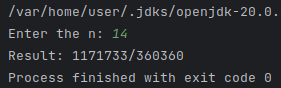
\includegraphics[scale=1]{1}
		\caption{Робота програми}
	\end{figure}

	\section*{Висновок}
	Під час виконання лабораторної роботи я реалізував кілька класів для виконання завдання, два з яких узагальнюються спільним інтерфейсом. При цьому використав як примітивні типи, так і довгі числа, а також утиліту Scanner для зчитування користувацького вводу.
	 
\end{normalsize}
\end{document}
